
%(BEGIN_QUESTION)
% Copyright 2014, Tony R. Kuphaldt, released under the Creative Commons Attribution License (v 1.0)
% This means you may do almost anything with this work of mine, so long as you give me proper credit

Examine this schematic diagram of a protective relay system, from page 18 of {\it Protective Relays} by Victor H. Todd (published in 1922):

$$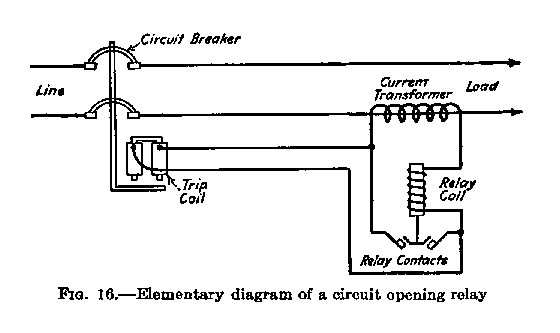
\includegraphics[width=15.5cm]{i03321x01.eps}$$

First, identify the modern ANSI/IEEE protective function number provided by this circuit.  Next, explain how it works, contrasting its design against modern protective relay systems of the same function.

\underbar{file i03321}
%(END_QUESTION)





%(BEGIN_ANSWER)

5 points for the ANSI/IEEE code, 5 points for the explanation.  Deduct 2 points if a correct explanation of this system is given, but with no contrast against modern 50 relay systems.

\vskip 10pt

This is a 50 (instantaneous overcurrent) protective relay.  Its operation differs from modern 50 relays in that it uses the CT's output as the power source for the circuit breaker's trip coil, rather than 125 VDC station power.  If the line current exceeds the relay's pick-up value, the relay contacts will open and all the CT's secondary current will be thusly redirected to the breaker trip coil.

%(END_ANSWER)





%(BEGIN_NOTES)

{\bf This question is intended for exams only and not worksheets!}.

%(END_NOTES)


